\documentclass[]{article}

\usepackage{cite} % Add this line to include the cite package
% \usepackage[backref]{hyperref} % Add this line to include the hyperref package

\usepackage{amsmath} % Add this line to include the amsmath package
\usepackage{graphicx} % Add this line to include the graphicx package
\usepackage{fancyhdr}

\title{\textbf{Computer Vision homework 3}}
\author{Pan Changxun}
\date{April 2025}

\topmargin=-0.45in      %
\evensidemargin=0in     %
\oddsidemargin=0in      %
\textwidth=6.5in   
\textheight=9.0in       %
\headsep=0.25in 

\pagestyle{fancy}
\fancyhf{} % Clear all header and footer fields
\fancyhead[L]{Pan Changxun} % Left header
\fancyhead[C]{Computer Vision homework 3} % Center header
\fancyhead[R]{April 2025} % Right header
%\fancyfoot[L]{\leftmark} % Left footer
\fancyfoot[C]{\thepage} % Center footer
%\fancyfoot[R]{} % Right footer

\begin{document}
\maketitle

\section{3D Location Transformation}
\begin{enumerate}
	\item[a)] The intrinsic matrix is given by:
	\begin{equation}
		K = \begin{bmatrix}
			f_x & 0 & c_x \\
			0 & f_y & c_y \\
			0 & 0 & 1
		\end{bmatrix}
	\end{equation}
	When \(f_x = f_y = f = 721.5\) and \(c_x, c_y = (609.6, 172.9)\), the intrinsic matrix becomes:
	\begin{equation}
		K = \begin{bmatrix}
			721.5 & 0 & 609.6 \\
			0 & 721.5 & 172.9 \\
			0 & 0 & 1
		\end{bmatrix}
	\end{equation}
	\item[b)] We use the camera's coordinates: \(x\) means the right, \(y\) means the down, \(z\) means the forward. Then the equation of the ground plane in camera's coordinate system is \(y=1.7m\).
	\item[c)] We use the same camera's coordinate system as in part b). 
	When given a 2D point (x,y) in the image and suppose it lies on the ground (y=1.7m), we can find the corresponding 3D point in the camera's coordinate system using the following equations:
	\begin{equation}
		Y = 1.7m
	\end{equation}
	\begin{equation}
		Z = \frac{Y \cdot f_y}{y - c_y} = \frac{1.7m \cdot 721.5}{y - 172.9}
	\end{equation}
	\begin{equation}
		X = Y \cdot \frac{x - c_x}{y - c_y} = 1.7m \cdot \frac{x - 609.6}{y - 172.9}
	\end{equation}
	where (X, Y, Z) are the coordinates of the corresponding 3D point in the camera's coordinate system and \(c_x, c_y\) equals to (609.6, 172.9).
\end{enumerate}

\section{Road Analyzing}
\begin{enumerate}
	\item[a)] For the depth map visualization, I truncated the 5\% most distant pixels to enhance the details of nearer objects. This approach provides better contrast and clarity in the depth representation.
		The resulting depth maps are stored in the folder "/src/problem2\_analyzing/data/depth/" with corresponding colorbars. An example depth map is shown below:
		\begin{figure}[h]
			\centering
			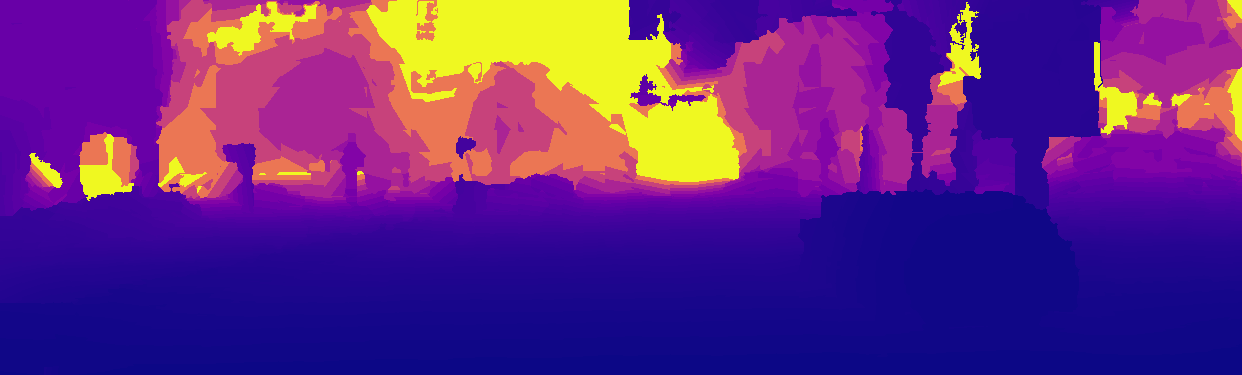
\includegraphics[width=0.5\textwidth]{src/problem2_analyzing/data/depth/004945_depth.png}
			\caption{Depth map visualization for frame 004945}
			\label{fig:depth_map_example}
		\end{figure}
		\newpage
		The corresponding colorbar for interpreting the depth values:
		\begin{figure}[h]
			\centering
			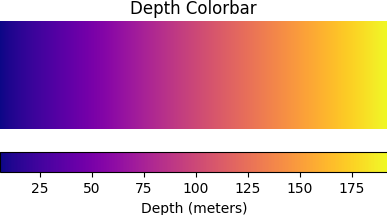
\includegraphics[width=0.5\textwidth]{src/problem2_analyzing/data/depth/004945_colorbar.png}
			\caption{Colorbar for depth map 004945}
			\label{fig:colorbar}
		\end{figure}
		
	\item[b)] The bounding box visualizations are stored in "/src/problem2\_analyzing/data/bbox/". A representative example is shown here:
		\begin{figure}[h]
			\centering
			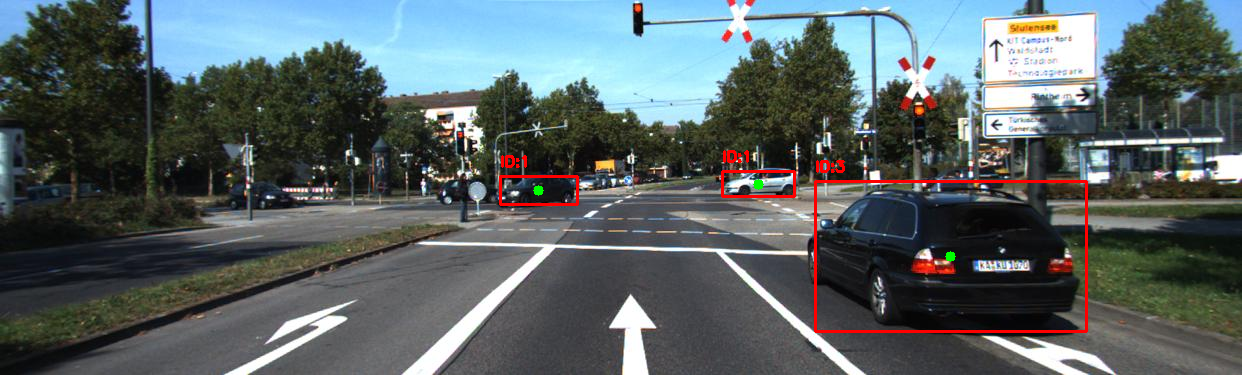
\includegraphics[width=0.5\textwidth]{src/problem2_analyzing/data/bbox/004945_bbox.png}
			\caption{Bounding box visualization for frame 004945}
			\label{fig:bbox_visualization}
		\end{figure}
		
		The calculated 3D coordinates for the centers of the bounding boxes are stored in "/src/problem2\_analyzing/data/3d\_coordinates/". Selected examples from frame 004945:
		
		\begin{center}
			\begin{tabular}{|c|c|c|}
				\hline
				\textbf{ID} & \textbf{2D coordinates} & \textbf{3D coordinates (meters)} \\
				\hline
				3 & [950, 256] & [3.239, 0.791, 6.864] \\
				1 & [758, 184] & [9.885, 0.742, 48.046] \\
				1 & [538, 190] & [-3.465, 0.830, 34.943] \\
				\hline
			\end{tabular}
		\end{center}
\end{enumerate}

\newpage
\section{Self-driving Detection (Bonus)}
The results are stored in "/src/problem3\_driving/output/". \\
Here are the keypoints of the self-driving detection algorithm:
% two figures
\begin{figure}[h]
	\centering
	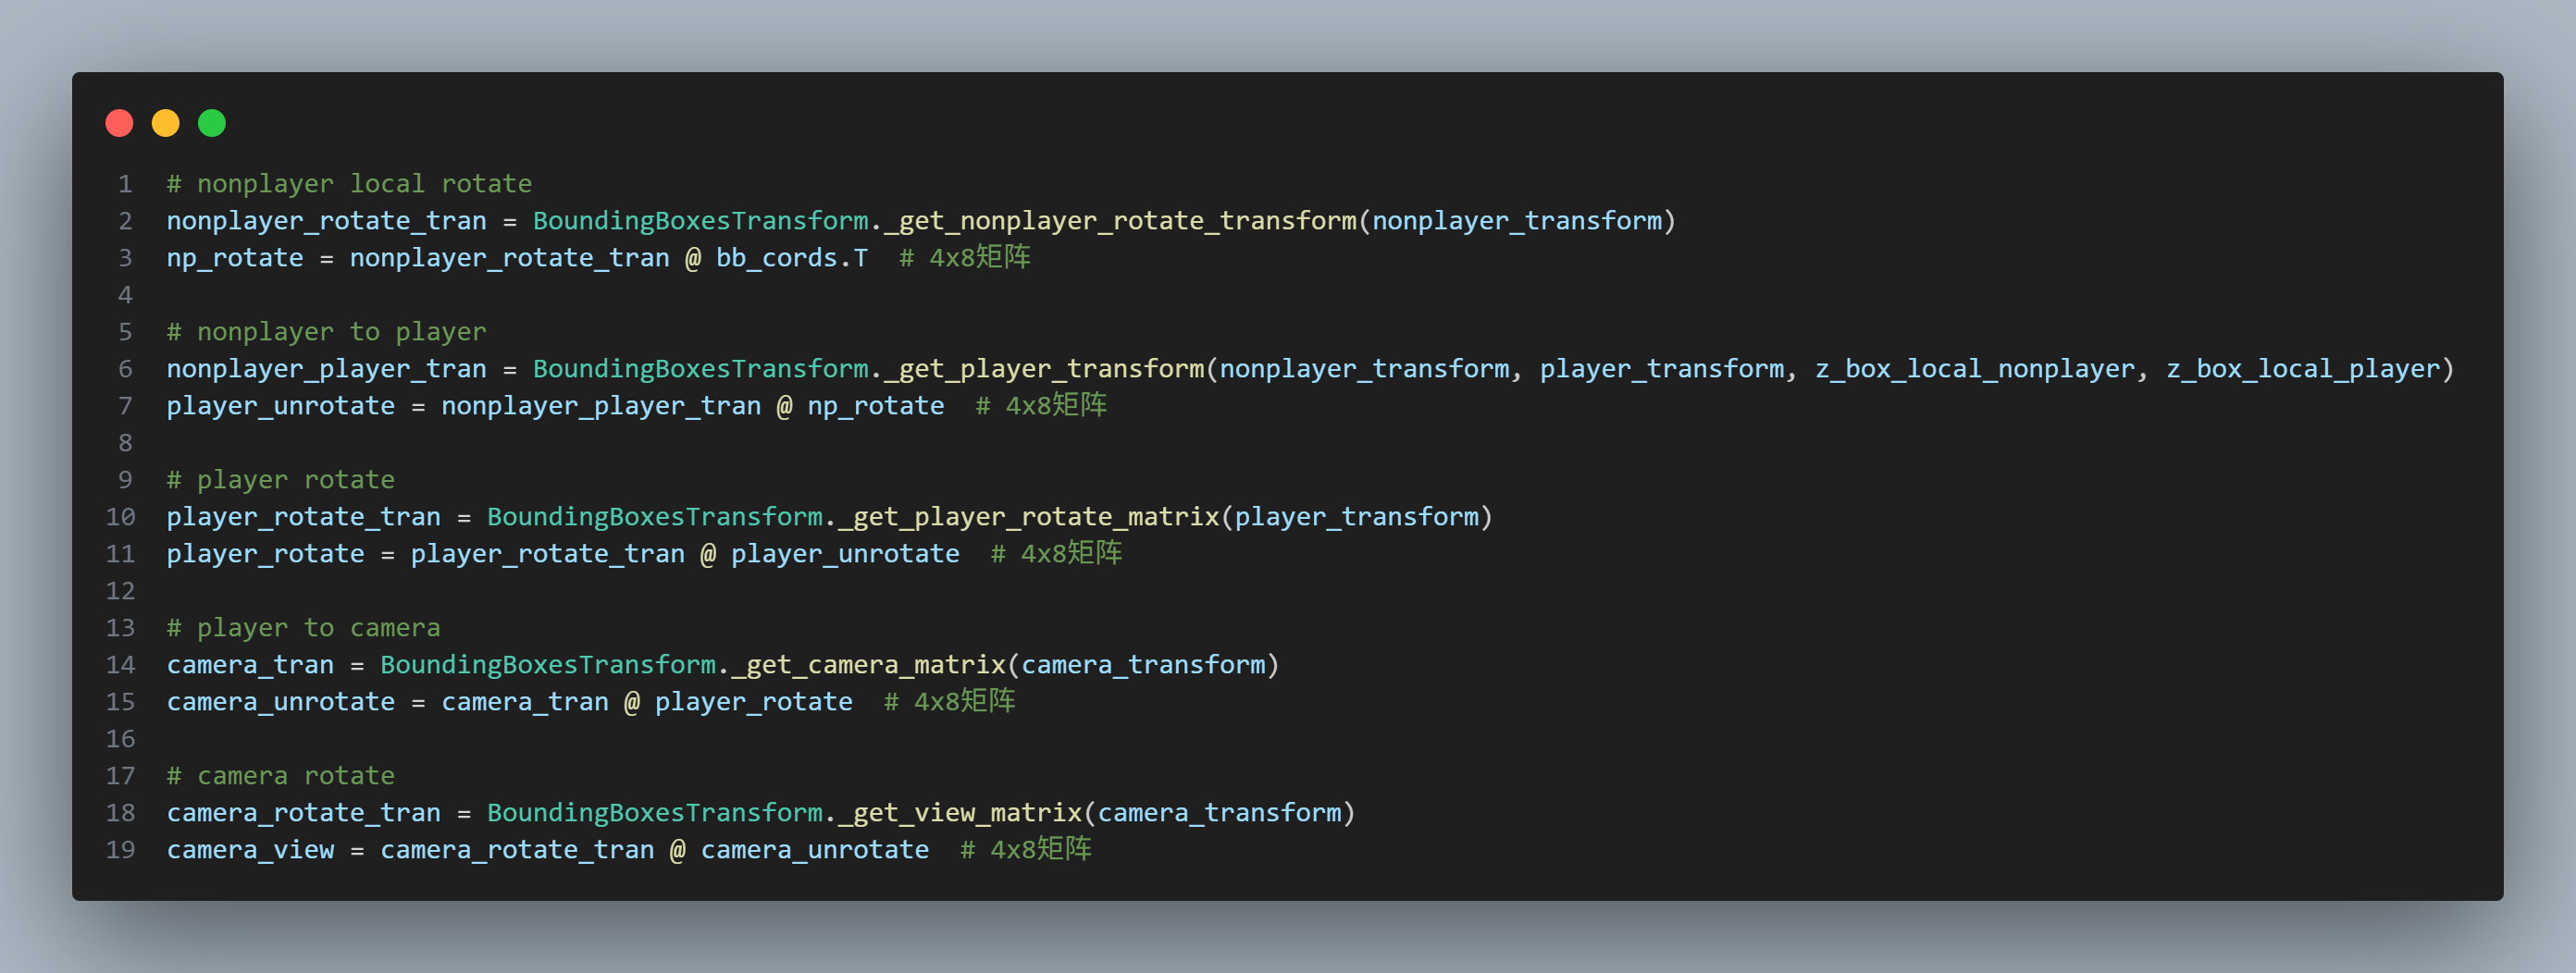
\includegraphics[width=1.0\textwidth]{pre1.png}
	\caption{}
	\label{fig:self_driving_keypoints}
\end{figure}
\begin{figure}[h]
	\centering
	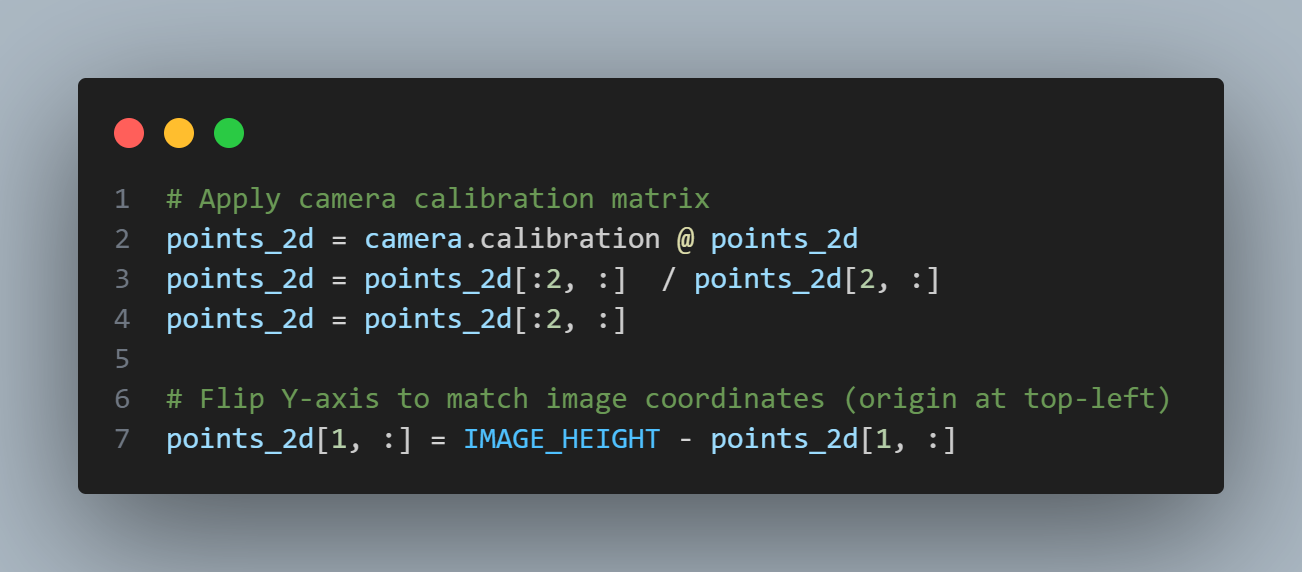
\includegraphics[width=0.5\textwidth]{pre2.png}
	\caption{}
	\label{fig:self_driving_3d_keypoints}
\end{figure}
\newpage
Here are the results of the self-driving detection algorithm: (3 figures)
\begin{figure}[h]
	\centering
	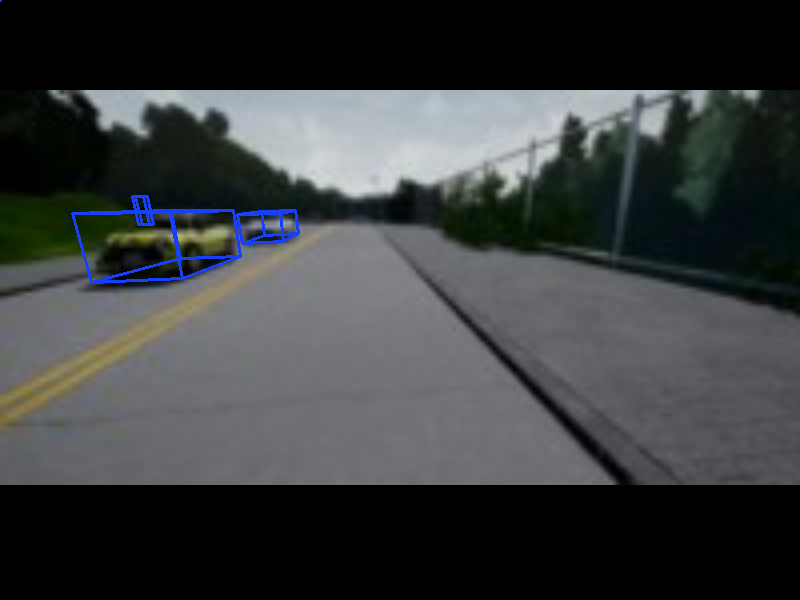
\includegraphics[width=0.5\textwidth]{src/problem3_driving/output/test_0.png}
	\caption{}
	\label{fig:self_driving_results_1}
\end{figure}
\begin{figure}[h]
	\centering
	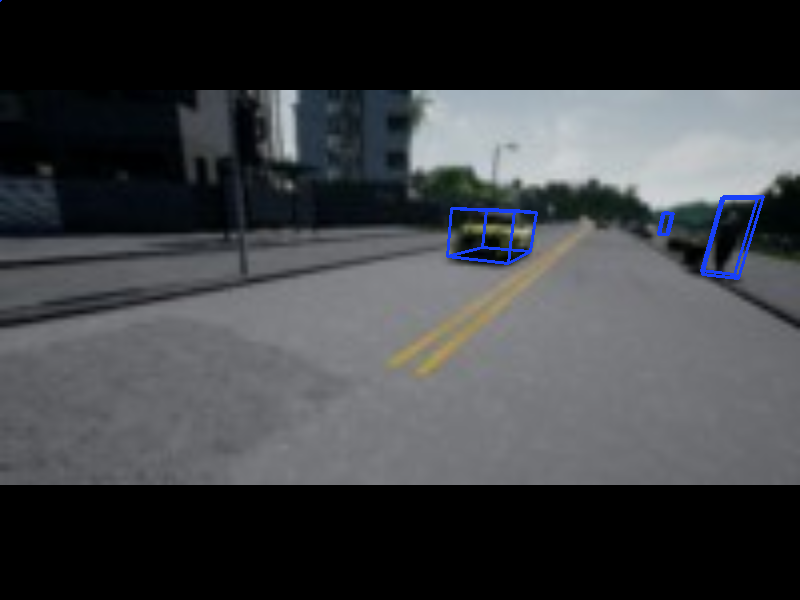
\includegraphics[width=0.5\textwidth]{src/problem3_driving/output/test_1.png}
	\caption{}
	\label{fig:self_driving_results_2}
\end{figure}
\begin{figure}[h]
	\centering
	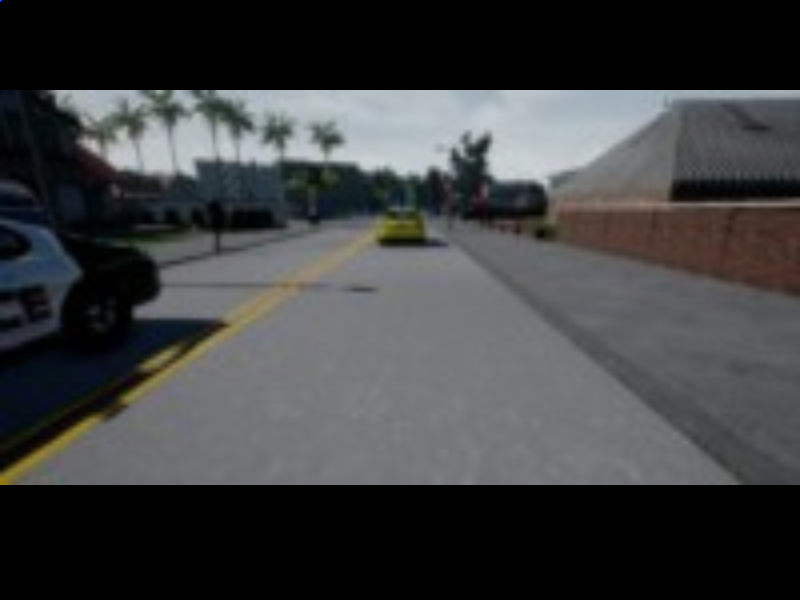
\includegraphics[width=0.5\textwidth]{src/problem3_driving/output/test_2.png}
	\caption{}
	\label{fig:self_driving_results_3}
\end{figure}

\end{document}